%(BEGIN_QUESTION)
% Copyright 2009, Tony R. Kuphaldt, released under the Creative Commons Attribution License (v 1.0)
% This means you may do almost anything with this work of mine, so long as you give me proper credit

Read and outline the ``Periodic Table of the Elements'' section of the ``Chemistry'' chapter in your {\it Lessons In Industrial Instrumentation} textbook.  Note the page numbers where important illustrations, photographs, equations, tables, and other relevant details are found.  Prepare to thoughtfully discuss with your instructor and classmates the concepts and examples explored in this reading.

\underbar{file i04097}
%(END_QUESTION)





%(BEGIN_ANSWER)


%(END_ANSWER)





%(BEGIN_NOTES)

Elements are the building-blocks of all substances.  Each element is defined by the number of protons in the nucleus of an atom.  This {\it atomic number} is always a whole-number quantity.  The {\it atomic mass} or {\it atomic weight} of an atom is the total number of protons + neutrons in the nucleus.  Elements with differing numbers of neutrons are called {\it isotopes}, sharing common chemical properties but differing in mass and in nuclear properties (e.g. radioactivity).

\vskip 10pt

A Periodic Table is called ``periodic'' because of the pattern represented by each row (period) in the table.  Elements in the same vertical column (group) tend to exhibit similar chemical properties (e.g. engage in similar sorts of chemical reactions).  The {\it first ionization energy} for each element is the amount of energy required to force an electrically neutral atom to become a positive ion (i.e. remove its first electron by force).  The greater this energy level, the more chemically ``stable'' an atom is.  A graph of first ionization energies showing the energy level required for ionization plotted against atomic number shows a repetitive ``sawtooth'' shape whereby the first group in each period of the Periodic Table is a low value, generally increasing in value until it reaches its peak in the last group of the period.  Group 1 elements such as lithium are readily ionized, and are highly reactive.  Group 18 elements such as argon are ``noble'' and are so stable they generally do not engage in chemical reactions at all.  Group 17 elements such as chlorine are just one electron shy of being as stable as a noble element, and so readily accumulate an extra electron in order to negatively ionize. 


\vskip 20pt \vbox{\hrule \hbox{\strut \vrule{} {\bf Suggestions for Socratic discussion} \vrule} \hrule}

\begin{itemize}
\item{} Explain why the Periodic Table of the Elements is aptly called ``periodic.''
\item{} Explain why atomic mass values given in a Periodic Table of the Elements are not whole numbers, despite the fact that the atomic mass of any atom is the sum of its protons and neutrons which must be whole-number quantities.
\item{} Explain how to make {\it pure water} radioactive.
\item{} Explain what {\it periodicity} means for chemical elements.
\item{} Identify which elements in the Periodic Table most readily {\it lose} an electron (i.e. become positively ionized).
\item{} Identify which elements in the Periodic Table most readily {\it gain} an electron (i.e. become negatively ionized).
\item{} Identify which elements in the Periodic Table have the most stable (i.e. lowest-energy) electron configuration.
\item{} Explain why Group 1 elements tend to bond readily with Group 17 elements, and how that bond is formed.
\item{} Group 16 elements are just {\it two} electrons shy of a noble configuration.  Given this fact, identify bonds that might form between any Group 16 elements and {\it two} atoms of Group 1 elements.
\item{} Explain what it means for an element to be ``noble'' in the chemical sense of the word.
\item{} Identify at least one compound that may be formed from a Group 1 element and a Group 17 element.
\item{} Looking at the first ionization energy graph, identify the elements just prior to each periodic peak and immediately following each periodic peak.
\item{} Looking at the first ionization energy graph, identify where all the Group 1 elements are found.
\item{} Looking at the first ionization energy graph, identify where all the Group 17 elements are found.
\item{} Looking at the first ionization energy graph, identify where all the Group 18 (``noble'') elements are found.
\end{itemize}














\vfil \eject

\noindent
{\bf Summary Quiz:}

The entry for {\it Potassium} in a Periodic Table of the Elements looks something like this:

$$\includegraphics[width=15.5cm]{i04097x01.eps}$$

From this entry, determine the number of protons and neutrons in a typical Potassium atom's nucleus:

\begin{itemize}
\item{} Protons = 19 ; Neutrons = 58
\vskip 5pt 
\item{} Protons = 19 ; Neutrons = 39 
\vskip 5pt 
\item{} Protons = 58 ; Neutrons = 20 
\vskip 5pt 
\item{} Protons = 19 ; Neutrons = 20
\vskip 5pt 
\item{} Protons = 20 ; Neutrons = 19 
\vskip 5pt 
\item{} Protons = 20 ; Neutrons = 39 
\end{itemize}

%INDEX% Reading assignment: Lessons In Industrial Instrumentation, Chemistry (periodic table of the elements)

%(END_NOTES)


